\documentclass[captions=tableheading]{scrartcl}

\usepackage{amsmath}
\usepackage{amssymb}
\usepackage[utf8]{inputenc}
\usepackage[T1]{fontenc}
\usepackage{lmodern}
\usepackage{ngerman}
\usepackage{geometry}
\usepackage{graphicx}
\usepackage{wrapfig}
\usepackage{caption}
\usepackage{wasysym}
\usepackage[separate-uncertainty=true]{siunitx}
\usepackage{picinpar}
\usepackage{tikz}
\usepackage{float}
\usepackage{booktabs}
\usepackage{enumitem} 

\renewcommand{\figurename}{Abb.}
\usepackage[
	colorlinks=true,
	urlcolor=blue,
	linkcolor=black
]{hyperref}


%Hier Titel und so
\newcommand{\versuchnummer}{V27} 
\newcommand{\versuchname}{Der Zeeman-Effekt} 
\newcommand{\versuchdatum}{16.02.2017} 
\newcommand{\im}{\mathrm{i}}
\newcommand{\indx}[1]{\text{#1}}
\newcommand{\RE}[1]{\mathrm{Re} \left(#1 \right)}


\title{Versuch \versuchnummer\\ \versuchname}
\subtitle{Physikalisches Fortgeschrittenenpraktikum}
\author{Robert Rauter und Björn Lindhauer}
\date{\versuchdatum} 
\begin{document}
\begin{titlepage}
{\large \versuchdatum}
\vspace{7cm}
\begin{center}
\textbf{\huge Versuch \versuchnummer}\\\vspace{0.5cm}
\textbf{\huge \versuchname}\\
\vspace{0.2cm}
\textbf{Physikalisches Fortgeschrittenenpraktikum}\\
\vspace{9cm}

{\Large Robert Rauter \ \ \hspace{1.5cm} und \hspace{1.5cm} Björn Lindhauer}\\
{ \url{robert.rauter@tu-dortmund.de} \ \ \hspace{2cm} \url{bjoern.lindhauer@tu-dortmund.de}}
\end{center}
\end{titlepage}

\section{Theoretische Grundlagen}
Unter den Zeeman-Effekt wird die Aufspaltung der Spektrallinien von Atomen unter Einfluss eines äußeren Magnetfelds verstanden. 
Es können dabei Aussagen über die Energien und Polarisation der Spektrallinien anhand von Auswahlregeln gemacht werden.

\subsection{Magnetische Moment eines Elektrons}
Elektronen besitzen einen Bahndrehimpuls $\vec{l}$ und Eigendrehimpuls $\vec{s}$, der auch Spin genannt wird, welche über die Quantenzahlen $l$ bzw. $s$
\begin{align}
\left| \vec{l} \right| &= \sqrt{l\left(l+1\right)}\hbar &  \text{mit } l=0,1,...,n-1\\
\left| \vec{s} \right| &= \sqrt{s\left(s+1\right)}\hbar &  \text{mit }  s=\frac{1}{2}
\end{align}
beschrieben werden können.

Da Elektronen geladene Teilchen sind, ist der Drehimpuls mit dem magnetischen Moment 
\begin{align}
\mu_\indx{z}=-\frac{1}{2}e_\indx{0} \frac{\hbar}{m_0}=:\mu_\indx{B}
\end{align}
verknüpft. 
Die Größe $\mu_\indx{B}$ wird als Bohrsche Magneton bezeichnet.

Es ergeben sich so zwei magnetische Momente
\begin{align}
\vec{\mu_\indx{l}}&=-\mu_\indx{B}\frac{\vec{l}}{\hbar}=-\mu_\indx{B}\sqrt{l\left(l+1\right)}\vec{e_\indx{l}}\\
\vec{\mu_\indx{s}}&=-g_\indx{s}\mu_\indx{B}\frac{\vec{s}}{\hbar}=-g_\indx{s}\mu_\indx{B}\sqrt{s\left(s+1\right)}\vec{e_\indx{s}}
\end{align}
mit den Einheitsvektoren $\vec{e_\indx{l}}$ in $\vec{l}$-Richtung und $\vec{e_\indx{s}}$ in $\vec{s}$-Richtung und den Landr\'{e}-Faktor $g_\indx{s}\approx 2$.
Die Eigenschaft $\mu_\indx{s}\approx 2\mu_\indx{l}$ wird als magnetomechanische Anomalie des Elektrons bezeichnet.
\subsection{Wechselwirkung der Drehimpulse und magnetischen Momente}
In einem Mehrelektronensystem wird die Wechselwirkung zwischen den beiden Drehimpulsen und magnetischen Momenten eines einzelnen Elektrons und zwischen verschiedenen Elektronen unterschieden.

Die Bahndrehimpulse können bei niedriger Kernladungszahl aufgrund ihrer starken Wechselwirkung zu einem Gesamtdrehimpuls
\begin{align}
\vec{L}=\sum \vec{l_i}
\end{align}
zusammengefasst werden.
Dabei werden nur Elektronen aus der äußersten, nicht abgeschlossenen Schale betrachtet, da volle Schalen nach der ersten Hundschen Regel Gesamtdrehimpuls null haben.
Auch die Spins können zu einem Gesamtspin
\begin{align}
\vec{S}=\sum \vec{s_i}
\end{align}
zusammengefasst werden.

Es kann analog zu den einzelnen Drehimpulsen eine Verknüpfung mit Quantenzahlen
\begin{align}
\left| \vec{L} \right| &= \sqrt{L\left(L+1\right)} &  \text{mit } L\in \mathbb{N}_{0}\\
\left| \vec{S} \right| &= \sqrt{S\left(S+1\right)} &  \text{mit }  s=\frac{N}{2},\frac{N}{2}-1,...,\frac{1}{2}, 0
\end{align}
gemacht werden. 
Dabei ist $N$ die Anzahl der Elektronen in der äußeren Schale.

Es können $\vec{L}$ und $\vec{S}$ zu einem Gesamtdrehimpuls
\begin{align}
\vec{J}=\vec{L}+\vec{S}
\end{align}
mit
\begin{align}
\left| \vec{J} \right| &= \sqrt{J\left(J+1\right)} \hspace{0.2cm}\text{.}
\end{align}
Dieser Zusammenhang bleibt auch für kleine Störungen durch äußere Magnetfelder gültig.

Bei Atomen mit größerer Kernladungszahl wird $\vec{J}$ aufgrund der hohen Wechselwirkung der Spins und der Bahndrehimpulse miteinander wird der Gesamtdrehimpuls durch die j-j-Kopplung
\begin{align}
\vec{j_i}=\vec{l_i}+\vec{s_i} \\
\vec{J}=\sum \vec{j_i}
\end{align}
bestimmt.
\subsection{Aufspaltung der Energieniveaus}
Im Allgemeinen ist das magnetische Moment
\begin{align}
\vec{\mu}=\vec{\mu_\indx{L}}+\vec{\mu_\indx{S}}
\end{align}
nicht parallel zu $\vec{J}$, sodass eine Unterscheidung in $\mu_{\perp}$ und $\mu_{\parallel}$ sinnvoll ist.
Es gilt außerdem für das magnetische Moment
\begin{align}
\left| \vec{\mu_\indx{J}} \right| &=\mu_\indx{B}g_\indx{J} \sqrt{J\left(J+1\right)}
\end{align}
mit dem Landr\'{e}-Faktor
\begin{align}
g_\indx{J}=\frac{3J\left(J+1\right)+S\left(S+1\right)-L\left(L+1\right)}{2J\left(J+1\right)}\hspace{0.2cm}\text{.}
\end{align}
Aus der Richtungsquantelung ergibt sich eine Orientierungsquantenzahl, die genau $2J+1$ Werte annehmen kann und somit genauso viele Einstellungsmöglichkeiten des magnetischen Moments relativ zur Richtung des äußeren Feldes gibt.
Die dabei auftretende Energie $E_\indx{mag}$ ist durch
\begin{align}
E_\indx{mag}=mg_\indx{J}\mu_\indx{B}\hspace{0.2cm}\text{mit }-J\le m \le J 
\end{align}
gegeben.

Das Energieniveau spaltet sich somit in $2J+1$ äquidistante Niveaus auf, wie in Abbildung \ref{fig:aufspaltungj2} dargestellt.

\begin{center}
	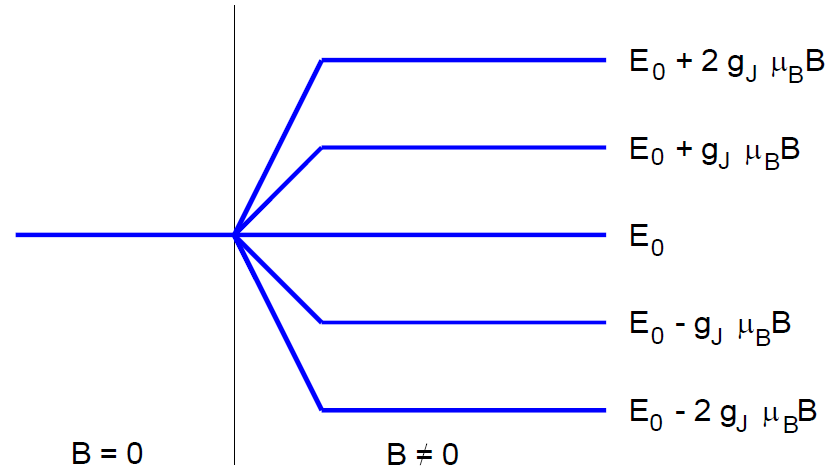
\includegraphics[width=10cm]{images/aufspaltungj2.png}
	\captionof{figure}{Aufspaltung eines Energieniveaus eines Atoms mit der Gesamtdrehimpulsquantenzahl $J=2$. \ref{q:anleitung}}
	\label{fig:aufspaltungj2}
\end{center}

Bei angeregten Atomen können Übergänge zwischen diesen zusätzlichen Energieniveaus angeregt werden, sodass eine einzelne Spektrallinie in mehrere Spektrallinien aufspaltet.
\subsection{Auswahlregeln für Übergänge zwischen zeemanaufgespaltenen Niveaus}
Aus der zeitabhängigen Schrödinger-Gleichung lässt sich eine zeitabhängige Dichteverteilung herleiten, die Schwingung der Elektronen mit der Frequenz
\begin{align}
\nu_{\alpha\beta}=\frac{E_\alpha-E_\beta}{h}
\end{align}
beschreibt.

Außerdem können nur Übergänge mit 
\begin{align}
\Delta m = m_\alpha - m_\beta = -1,\ 0 \text{ oder } 1
\end{align}
angeregt werden.
Dabei sind die bei $\Delta m=0$ emittierten Strahlen linear-polarisiert und parallel zu $\vec{B}$ und die bei $\left|\Delta m \right|=1$ zirkular-polarisiert um die z-Achse.
\subsection{Normale Zeeman-Effekt}
Der Normale Zeeman-Effekt betrachtet den Fall $S=0$. 
Es ergeben sich somit die Energieunterschiede
\begin{align}
\Delta E=m\mu_\indx{B}\hspace{0.2cm}\text{mit }-J\le m \le J \text{.}
\end{align}
Die möglichen Übergänge zwischen $J=2$ und $J=1$ sind in Abbildung \ref{fig:aufspaltungnormal} dargestellt.
\begin{center}
	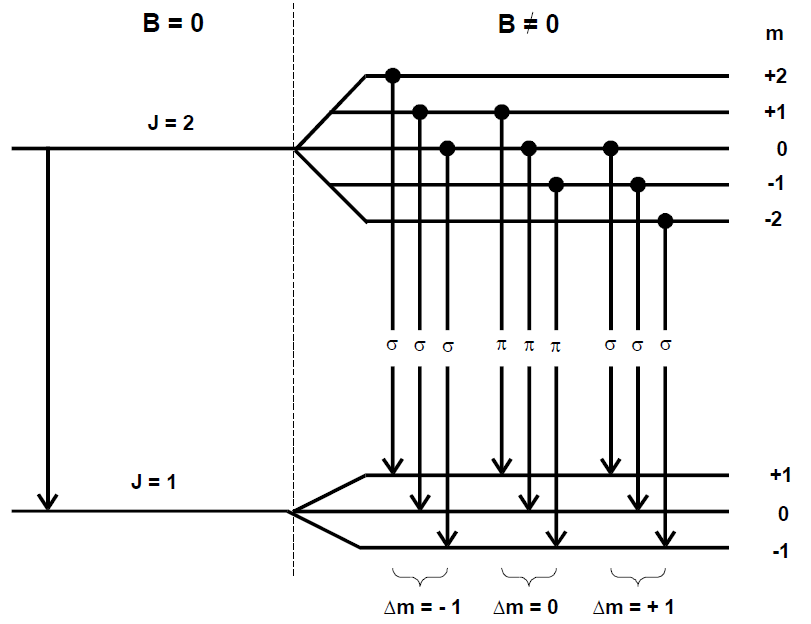
\includegraphics[width=10cm]{images/aufspaltungnormal.png}
	\captionof{figure}{Aufspaltung und Polarisation der Spektrallinien beim normalen Zeeman-Effekt zwischen $J=2$ und $J=1$. \ref{q:anleitung}}
	\label{fig:aufspaltungnormal}
\end{center}
Dabei ist $\Delta m=0$ die $\pi$-Komponente, welche nur bei senkrechter, transversalen Beobachtung zur Feldrichtung mit voller Intensität beobachtbar ist. 
Der Übergang mit $\Delta m=\pm 1$ wird als $\sigma$-Komponente bezeichnet und ist bei jeder Beobachtungsart zu sehen. 
In Abbildung \ref{fig:aufspaltungsbild} ist dieses Aufspaltungsbild visualisiert.
\begin{center}
	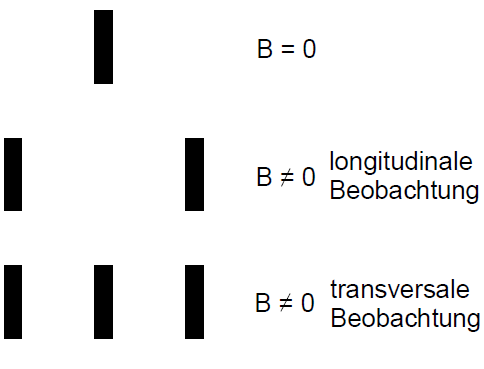
\includegraphics[width=7cm]{images/aufspaltungsbild.png}
	\captionof{figure}{Aufspaltungsbild einer Spektrallinie beim normalen Zeeman-Effekt. \ref{q:anleitung}}
	\label{fig:aufspaltungsbild}
\end{center}

\subsection{Anormale Zeeman-Effekt}
Beim anormalen Zeeman-Effekt wird $S\neq 0$ betrachtet. 
Die Energie zwischen einem Niveau mit Quantenzahlen $L_1$, $S_1$, $J_1$, $m_1$ und einem Niveau mit $L_2$, $S_2$, $J_2$, $m_2$ ist durch 
\begin{align}
E=\left[ m_1 g\left(L_1,S_1,J_1 \right) - m_2 g\left(L_2,S_2,J_2 \right) \right] \mu_\indx{B}B+E_0
\end{align}
gegeben.
Es ergibt sich somit eine linienreichere Aufspaltung, wie in Abbildung \ref{fig:aufspaltunganormal} dargestellt.
\begin{center}
	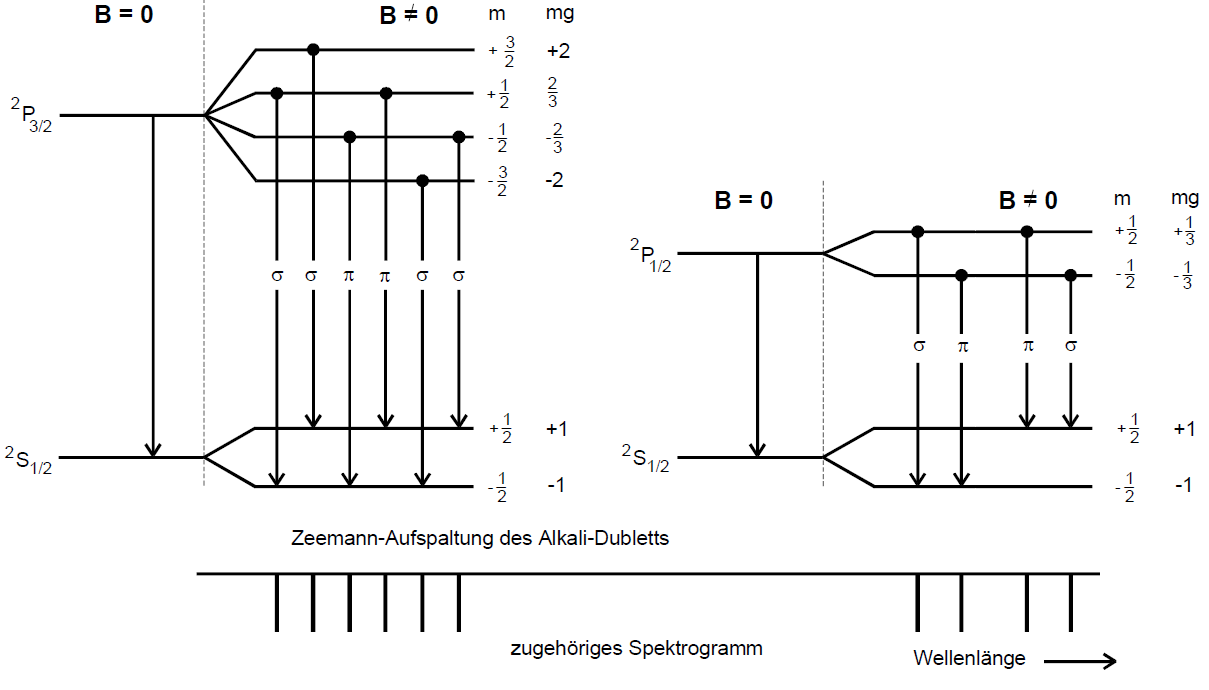
\includegraphics[width=12cm]{images/aufspaltunganormal.png}
	\captionof{figure}{Beispiel einer Linienaufspaltung beim anomalen Zeeman-Effekt. Dargestellt ist die Aufspaltung eines Alkali-Dubletts. \ref{q:anleitung}}
	\label{fig:aufspaltunganormal}
\end{center}

\section{Aufbau und Durchführung}
Der Versuchsaufbau ist in Abbildung \ref{fig:aufbau} dargestellt. 
\begin{center}
	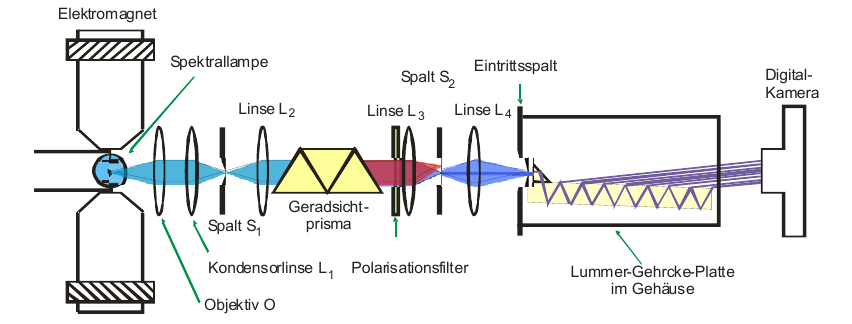
\includegraphics[width=\textwidth]{images/aufbau.png}
	\captionof{figure}{Schematische Darstellung des Versuchaufbaus}
	\label{fig:aufbau}
\end{center}
Für den Versuchsuafbau wird eine Cd-Lampe verwendet, die in das Magnetfeld eines Elektromagneten gestellt wird. 
\begin{center}
	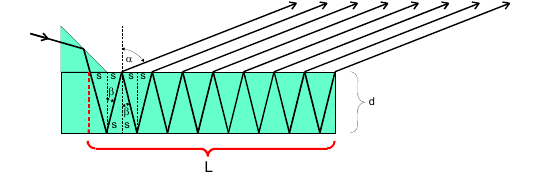
\includegraphics[width=\textwidth]{images/lummergercke.png}
	\captionof{figure}{Strahlengang in der Lummer-Gercke-Platte}
	\label{fig:lummergercke}
\end{center}
Die Lichtstrahlen werden mit mehreren Linsen und einem Spalt fokussiert und auf ein Geradsichtprisma gelenkt. Nachdem der Strahl durch das Prisma aufgespalten wird, kann mittels eines Polarisationsfilters und einem Spalt nach Wellenlänge und Polarisationsrichtung ausgewählt werden. \\
Weitere Linsen fokussieren den Strahl auf die Lummer-Gercke-Platte. Der Strahlengang in der Lummer-Gercke-Platte ist in Abbildung \ref{fig:lummergercke} dargestellt.
Durch Reflektion und Transmission entsteht ein Interferenzmuster, dessen Gangunterschied der eingehenden Wellenlänge entspricht. Beim Einschalten des Magnetfeldes verschiebt sich somit das Interferenzmuster um $\delta s$ und hat eine Wellenlängenänderung $\delta \lambda$ zur Folge, woraus die Landé-Faktoren bestimmt werden können. \\
Das Interferenzmuster wird dann mit einer Digitalkamera aufgenommen.\\
Zur Durchführung des Versuches muss zunächst der Strahlengang so justiert werden, dass am Ausgang des Gehäuses um die Lummer-Gercke-Platte ein klares Interferenzmuster zu erkennen ist. Dies wird mithilfe der grünen Spektrallinie durchgeführt. \\
Danach werden für die beiden Spektrallinien mit $\lambda=\SI{643.8}{\nano\metre}$ sowie $\lambda=\SI{480.0}{\nano\metre}$ Interferenzmuster mit und ohne angeschaltetem Magnetfeld aufgenommen. Im Falle der Spektrallinie mit $\lambda=\SI{480.0}{\nano\metre}$ wird dabei der Polarisationsfilter auf $0^{\circ}$ bzw. $90^{\circ}$ gestellt, um die jeweiligen Polarisationsrichtungen zu unterscheiden.

\section{Vorbereitung}

\subsection{Dispersionsgebiet und Auflösung der Lummer-Gercke-Platte}
\begin{table}[H]
	\centering
	\captionof{table}{Auflösungsvermögen A und Dispersionsgebiet $\Delta \lambda_D$ der Lummer-Gercke-Platte für die verwendeten Wellenlängen $\lambda$}
	\label{tab:lummer}
	\begin{tabular}{r r r}
		\toprule
		$\lambda$/nm & $\lambda_D$/pm & A \\
		\midrule
		643.8 & 48.9 & 209129 \\
		480.0 & 27.0 & 285458 \\
		\bottomrule
	\end{tabular}
\end{table}
In Tabelle \ref{tab:lummer} sind die Auflösungvermögen $A$ sowie die Dispersionsgebiete $\lambda_D$ für die verwendeten Wellenlängen aufgeführt.
Das Dispersionsgebiet berechnet sich dabei aus der Wellenlänge $\lambda$, dem Brechungsindex n und der Dicke der Platte d zu
\begin{align}
\Delta \lambda_D=\frac{\lambda^2}{2d}\sqrt{\frac{1}{n^2-1}}\,.
\end{align}
Die Auflösung der Lummer-Gercke wird mit der Länge der Platte L, der Wellenlänge $\lambda$ und mit em Brechungsindex n mithilfe der Gleichung
\begin{align}
A=\frac{L}{\lambda}\sqrt{n^2-1}
\end{align}
berechnet.
\subsection{Berechnung der Landé-Faktoren}
In Tabelle \ref{tab:landedrehimpuls} sind die Landé-Faktoren $g_i$ der verschiedenen Zustände mit den entsprechenden Drehimpulsquantenzahlen angegeben. \\
In Tabellen \ref{tab:landerot} und \ref{tab:landeblau} sind die daraus bestimmten Landé-Faktoren $g_{ij}$ der Übergänge im Magnetfeld angegeben.

\begin{table}[H]
	\centering
	\captionof{table}{Drehimpulsquantenzahlen sowie Landé-Faktoren der daraus resultierenden Zustände}
	\label{tab:landedrehimpuls}
	\begin{tabular}{r r r r r}
		\toprule
		Zustand & $l$ & $s$ & $j$ & $g_j$ \\
		\midrule
		$^1$P$_1$ & 1 & 0 & 1 & 1 \\
		$^1$D$_2$ & 2 & 0 & 1 & 1 \\
		$^3$P$_1$ & 1 & 0 & 1 & 1 \\
		$^3$S$_1$ & 0 & 1 & 1 & 1 \\
		\bottomrule	
	\end{tabular}
\end{table}

\begin{table}[H]
	\centering
	\captionof{table}{Landé-Faktoren $g_{ij}$ der Übergänge der Spektrallinien mit $\lambda=\SI{643.8}{\nano\metre}$ bei äußerem Magnetfeld}
	\label{tab:landerot}
	\begin{tabular}{r r r r r r}
		\toprule
		Übergang & $m_i$ & $g_i$ & $m_j$ & $g_j$ & $g_{ij}$ \\
		\midrule
		$\sigma^-$ & 2 & 1 & 1 & 1 & 1 \\
				   & 1 & 1 & 0 & 1 & 1 \\
				   & 0 & 1 & -1 & 1 &1 \\
		$\pi$	   & 1 & 1 & 1 & 1 & 0 \\
				   & 0 & 1 & 0 & 1 & 0 \\
				   & -1 & 1 & -1 & 1 & 0 \\
		$\sigma^+$ & 0 & 1 & 1 & 1 & -1 \\
				   & -1 & 1 & 0 & 1 & -1 \\
				   & -2 & 1 & -1 & 1 & -1 \\
		\bottomrule	
	\end{tabular}
\end{table}

\begin{table}[H]
	\centering
	\captionof{table}{Landé-Faktoren $g_{ij}$ der Übergänge der Spektrallinien mit $\lambda=\SI{480.0}{\nano\metre}$ bei äußerem Magnetfeld}
	\label{tab:landeblau}
	\begin{tabular}{r r r r r r}
		\toprule
		Übergang & $m_i$ & $g_i$ & $m_j$ & $g_j$ & $g_{ij}$ \\
		\midrule
		$\sigma^-$ & 1 & 1.5 & 0 & 2 & 1.5 \\
			   	   & 0 & 1.5 & -1 & 2 & 2 \\
		$\pi$	   & 1 & 1.5 & 1 & 2 & -0.5 \\
				   & 0 & 1.5 & 0 & 2 & 0 \\
				   & -1 & 1.5 & -1 & 2 & 0.5 \\
		$\sigma^+$ & 0 & 1.5 & 1 & 2 & -2 \\
				   & -1 & 1.5 & 0 & 2 & -1.5 \\
		\bottomrule	
	\end{tabular}
\end{table}

\section{Auswertung}

\subsection{Kalibrierung des Magnetfeldes}
Zur Bestimmung des Zusammenhanges zwischen Stromstärke und Magnetfeld wird für die Messwerte von Stromstärke und Magnetfeld eine lineare Ausgleichsrechung der Form
\begin{align}
B(I)=B_0+m\cdot I
\end{align}
durchgeführt. Die Messwerte sind in Tabelle \ref{tab:magnetfeld} dargestellt.
\begin{table}[H]
	\centering
	\captionof{table}{Magnetfeld $B$ in Abhängigkeit von $I$}
	\label{tab:magnetfeld}
	\begin{tabular}{r r}
		\toprule
		I / A & B / T \\
		\midrule
		0 & 0.004 \\
		1 & 0.058 \\
		2 & 0.115 \\
		3 & 0.171 \\
		4 & 0.228 \\
		5 & 0.285 \\
		6 & 0.343 \\
		7 & 0.403 \\
		8 & 0.453 \\
		9 & 0.512 \\
		10 & 0.564 \\
		11 & 0.630 \\
		12 & 0.675 \\
		13 & 0.733 \\
		14 & 0.785 \\
		15 & 0.836 \\
		16 & 0.869 \\
		17 & 0.910 \\ 
		18 & 0.936 \\
		19 & 0.962 \\
		20 & 0.988 \\
		\bottomrule
	\end{tabular}
\end{table}
Die Ausgleichsrechnung wird mithilfe von \textit{Python} durchgeführt und ergibt folgende Parameter:
\begin{align*}
B_0&=\SI{0.031(12)}{\tesla} \\
m&=\SI{0.0515(10)}{\tesla\per\ampere}
\label{eq:parameter}
\end{align*}
Die aufgenommenen Messdaten und der lineare Fit sind in Abbildung \ref{fig:magnetfeld} dargestellt.
\begin{center}
	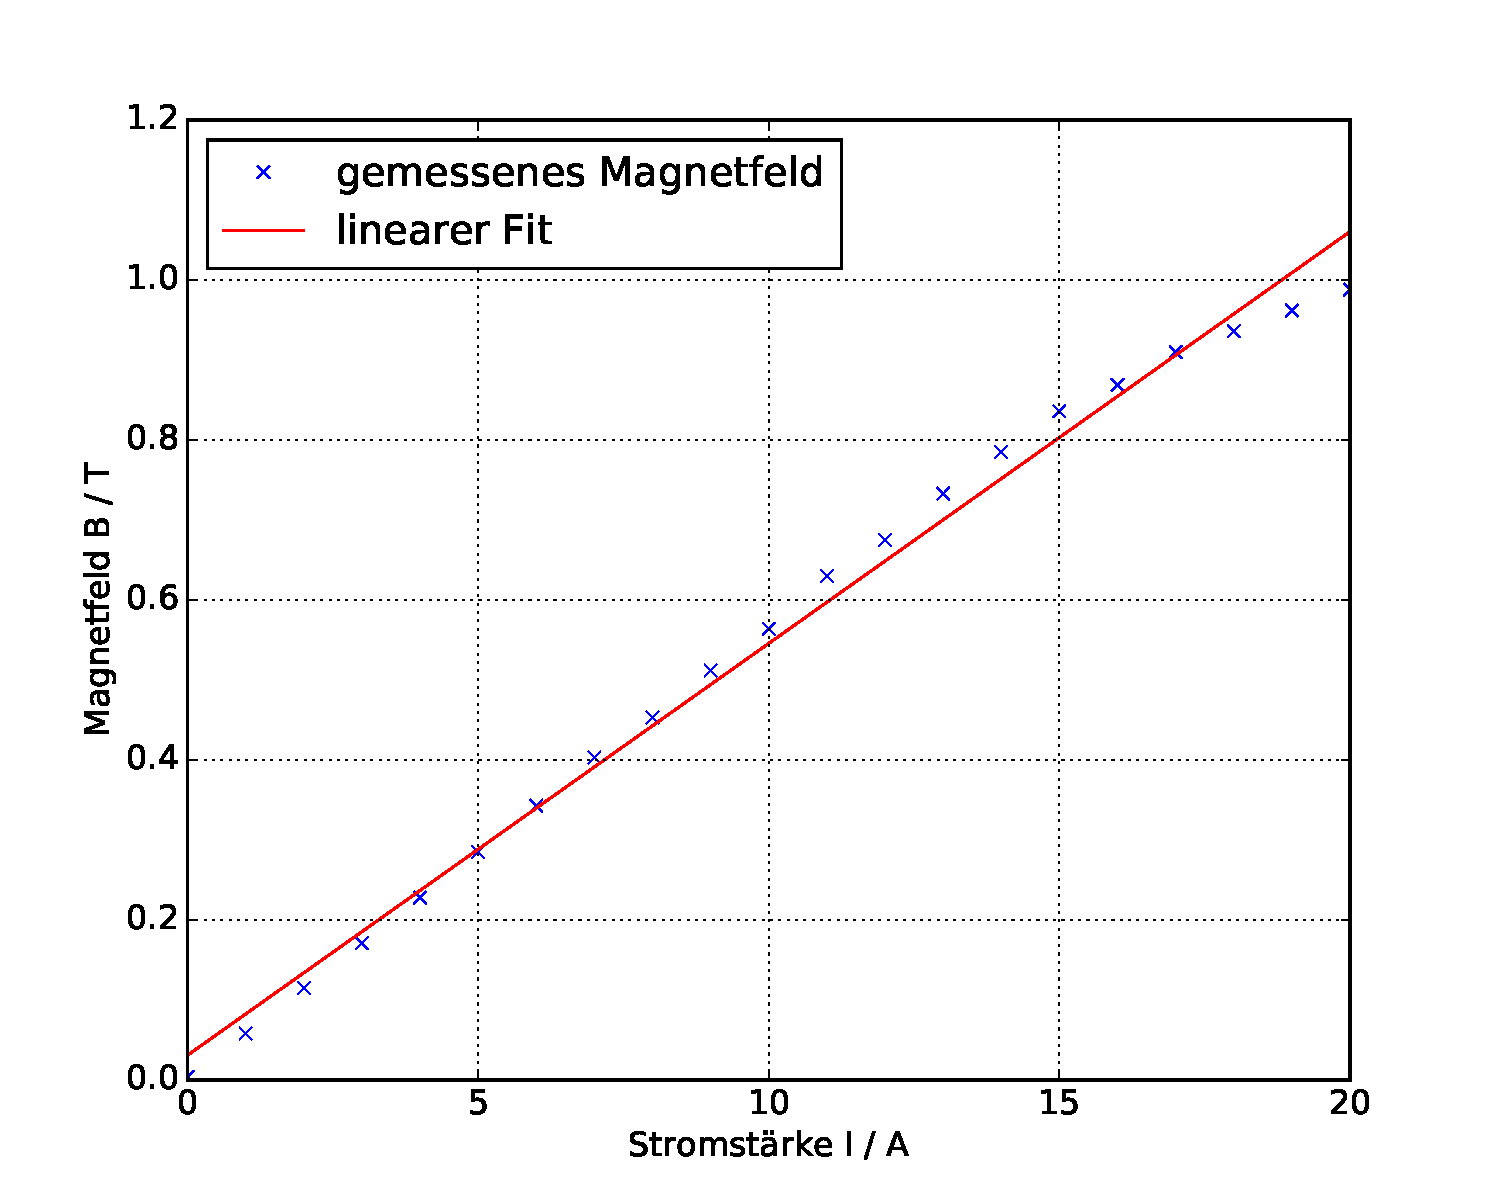
\includegraphics[width=0.8\textwidth]{images/magnetfeld.pdf}
	\captionof{figure}{Gemessenes Magnetfeld in Abhängigkeit von der Stromstärke und linearer Fit}
	\label{fig:magnetfeld}
\end{center}

\subsection{Bestimmung der Wellenlängenänderung}
Die Wellenlängenänderung $\delta\lambda$ ergibt sich aus der Gleichung
\begin{align}
\delta\lambda=\frac{1}{2}\frac{\delta s}{\Delta s}\Delta\lambda_{\text{D}},
\end{align}
wobei $\Delta s$ der Abstand der Interferenzstreifen ohne Magnetfeld, $\delta s$ der Abstand der Interferenzstreifen mit Magnetfeld und $\Delta\lambda_{\text{D}}$ das Dispersionsgebiet sind.

\subsubsection{$\sigma$-Übergänge für $\lambda=\SI{643.8}{\nano\metre}$}
\noindent\makebox[\textwidth][c]{
	\begin{minipage}[t]{0.6\textwidth}
		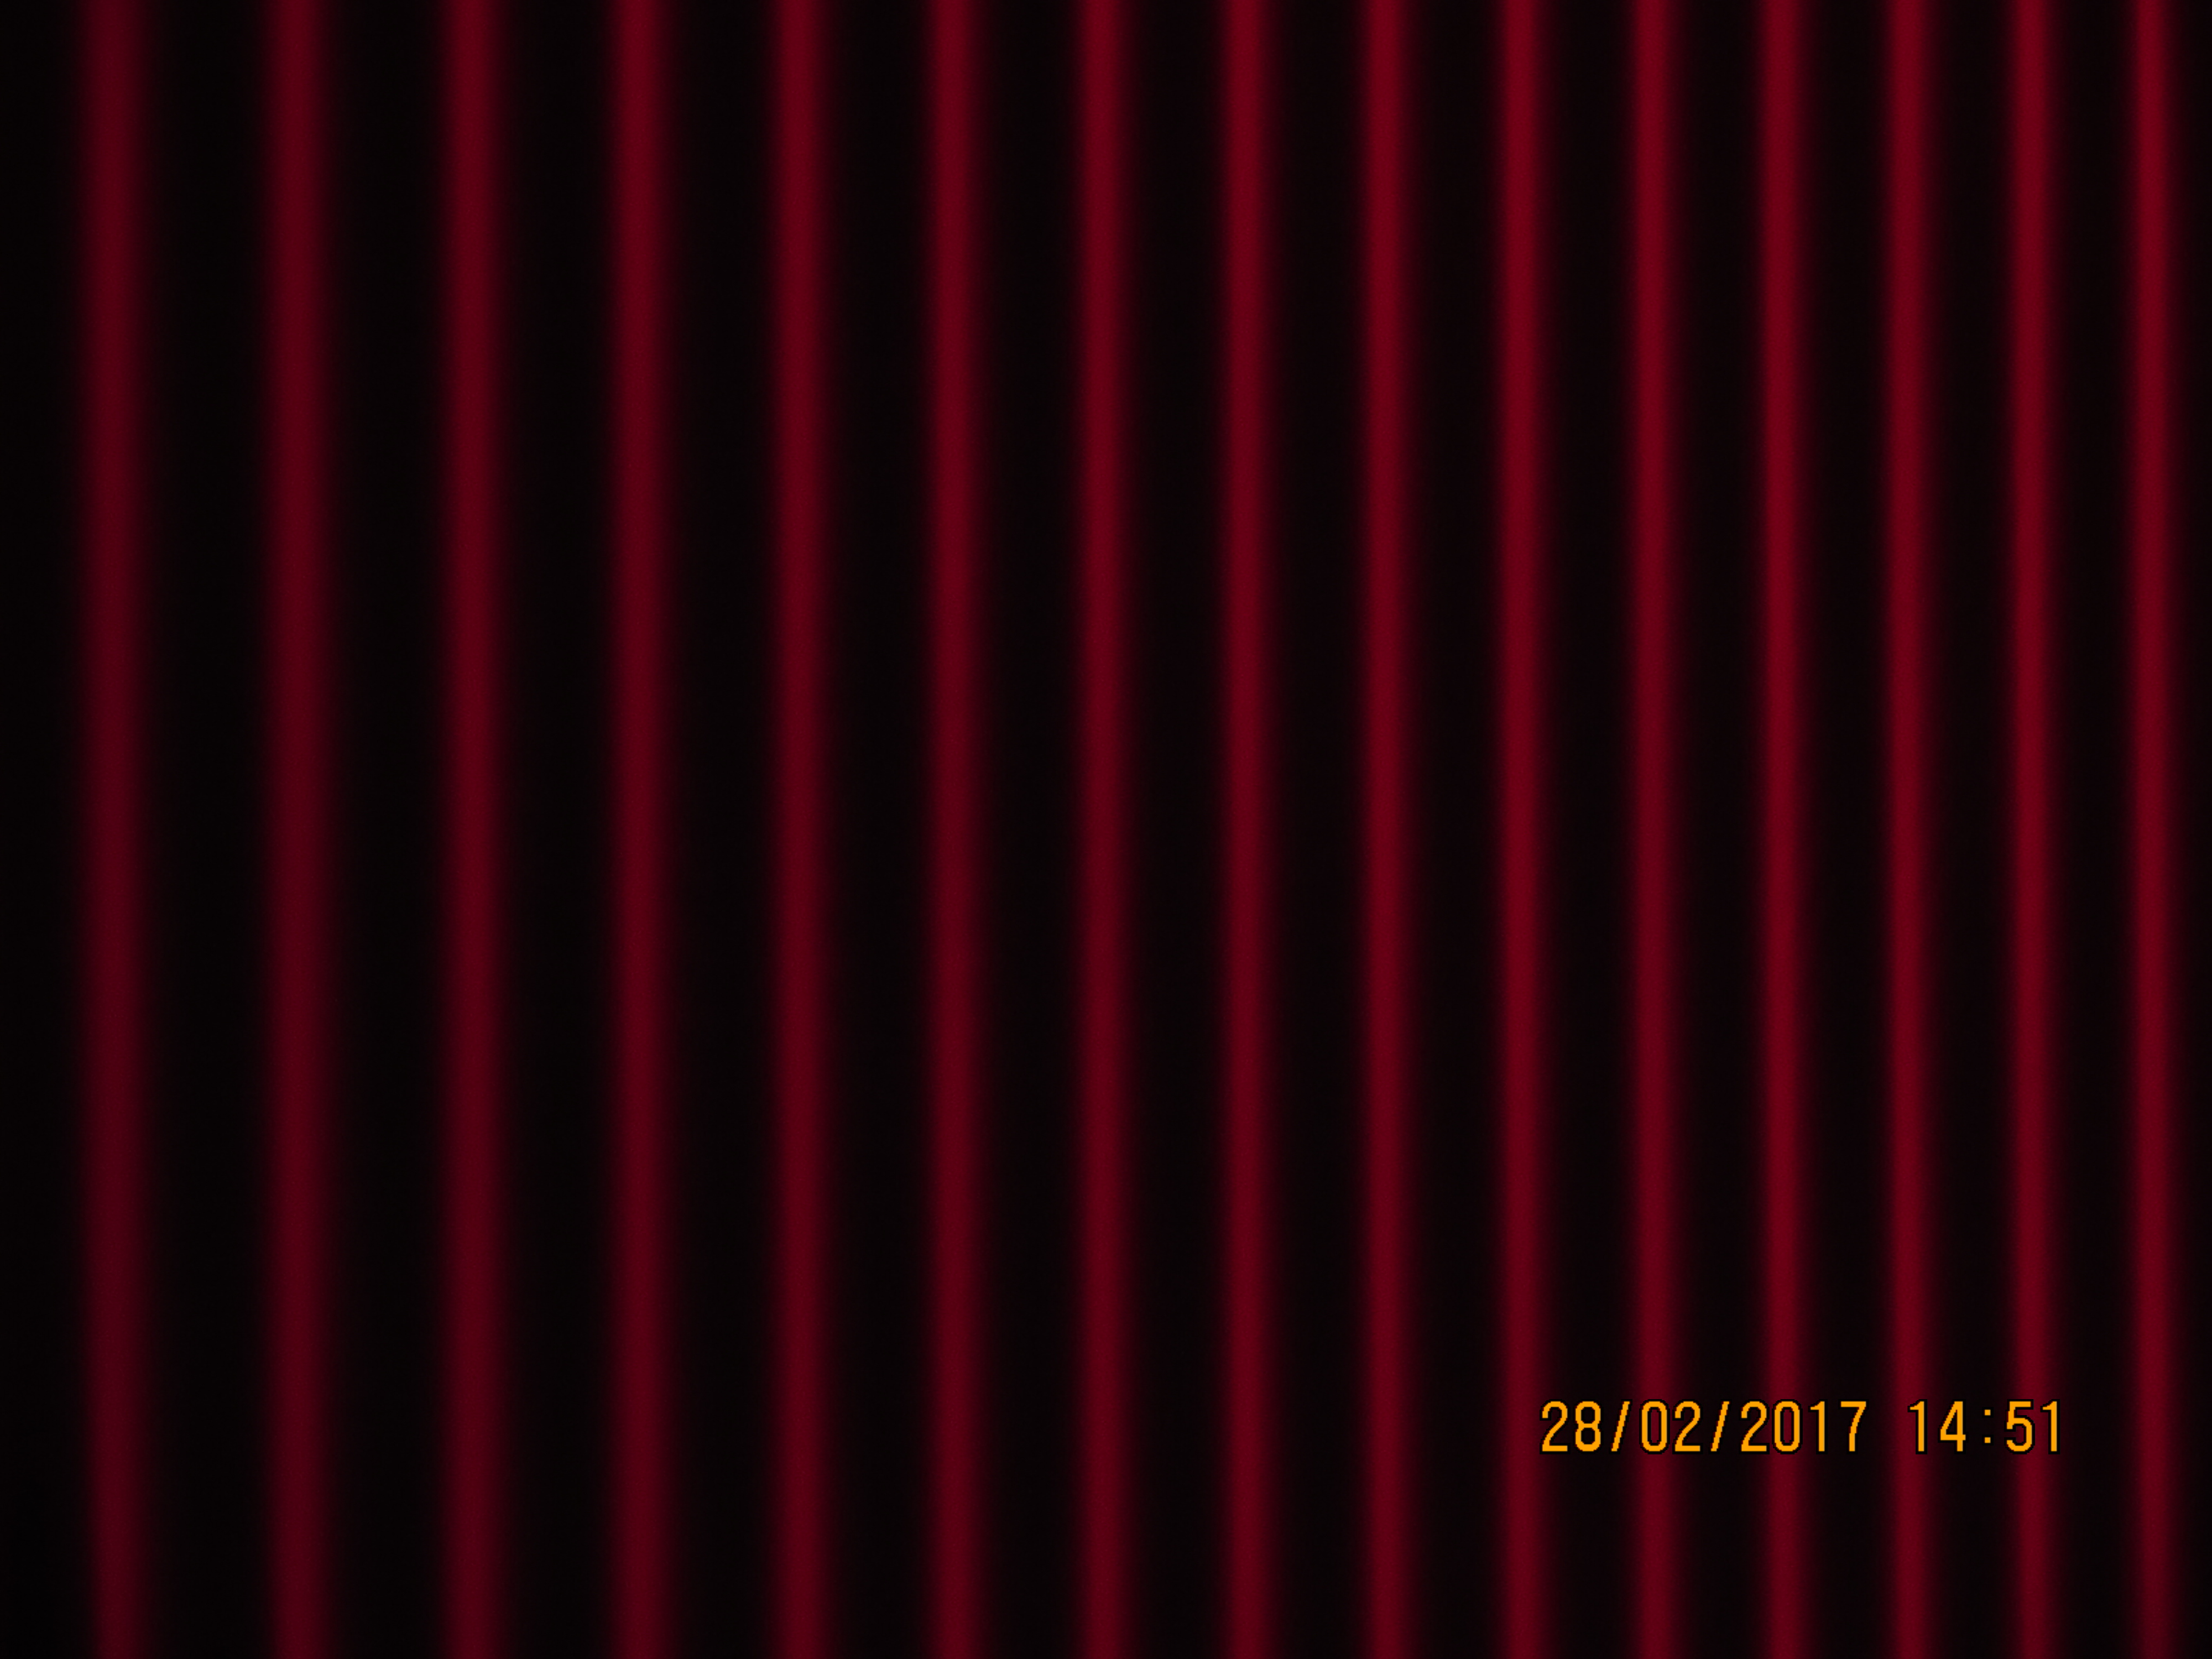
\includegraphics[width=\linewidth]{images/rot_oM.jpg}
		\centering
		a) B = $\SI{0}{\tesla}$
	\end{minipage}
	\begin{minipage}[t]{0.6\textwidth}
		
\includegraphics[width=\linewidth]{images/rot_mM.jpg}
		\centering
		b) B = $\SI{622.93}{\milli\tesla}$
	\end{minipage}}
\captionof{figure}{Interferenzmuster der Lummer-Gercke-Platte für die $\sigma$-Übergänge der Cd-Spektrallinie bei $\lambda=\SI{643.8}{\nano\metre}$, mit a) ohne Magnetfeld und b) mit Magnetfeld}
\label{fig:rot_sigma}
\vspace{0.5cm}
In Tabelle \ref{tab:rotmessung} sind die aus Abbildung \ref{fig:rot_sigma} abgelesenen Werte für $\delta s$ und $\Delta s$ sowie die daraus berechneten Wellenlängenänderungen dargestellt.
\begin{table}[H]
	\centering
	\captionof{table}{Abstände $\Delta s$ und $\delta s$ der Interferenzstreifen mit Wellenlängenänderung für die $\sigma$-Übergänge der Cd-Spektrallinie bei $\lambda=\SI{643.8}{\nano\metre}$}
	\label{tab:rotmessung}
	\begin{tabular}{r r r r}
		\toprule
		Ordnung n & $\Delta s$/px & $\delta s$/px & $\delta \lambda$/pm \\
		\midrule
		0 & 334 & 143 & 10.47 \\
		1 & 316 & 131 & 10.14 \\
		2 & 304 & 129 & 10.38 \\
		3 & 292 & 125 & 10.47 \\
		4 & 280 & 117 & 10.22 \\
		5 & 268 & 115 & 10.49 \\
		6 & 260 & 117 & 10.34 \\
		7 & 254 & 107 & 10.30 \\
		8 & 248 & 104 & 10.25 \\
		9 & 242 & 100 & 10.10 \\
		10 & 236 & 99 & 10.26 \\
		11 & 232 & 97 & 10.22 \\
		12 & 228 & 93 & 9.973 \\
		13 & 222 & 93 & 10.24 \\
		\bottomrule
	\end{tabular}
\end{table}
Der über mehrere Ordnungen gemittelte Wert der Wellenlängenänderung beträgt
\begin{align}
\delta \lambda = \SI{10.28(4)}{\pico\metre}\,.
\end{align}

\subsubsection{$\sigma$-Übergänge für $\lambda=\SI{480.0}{\nano\metre}$}

\noindent\makebox[\textwidth][c]{
	\begin{minipage}[t]{0.6\textwidth}
		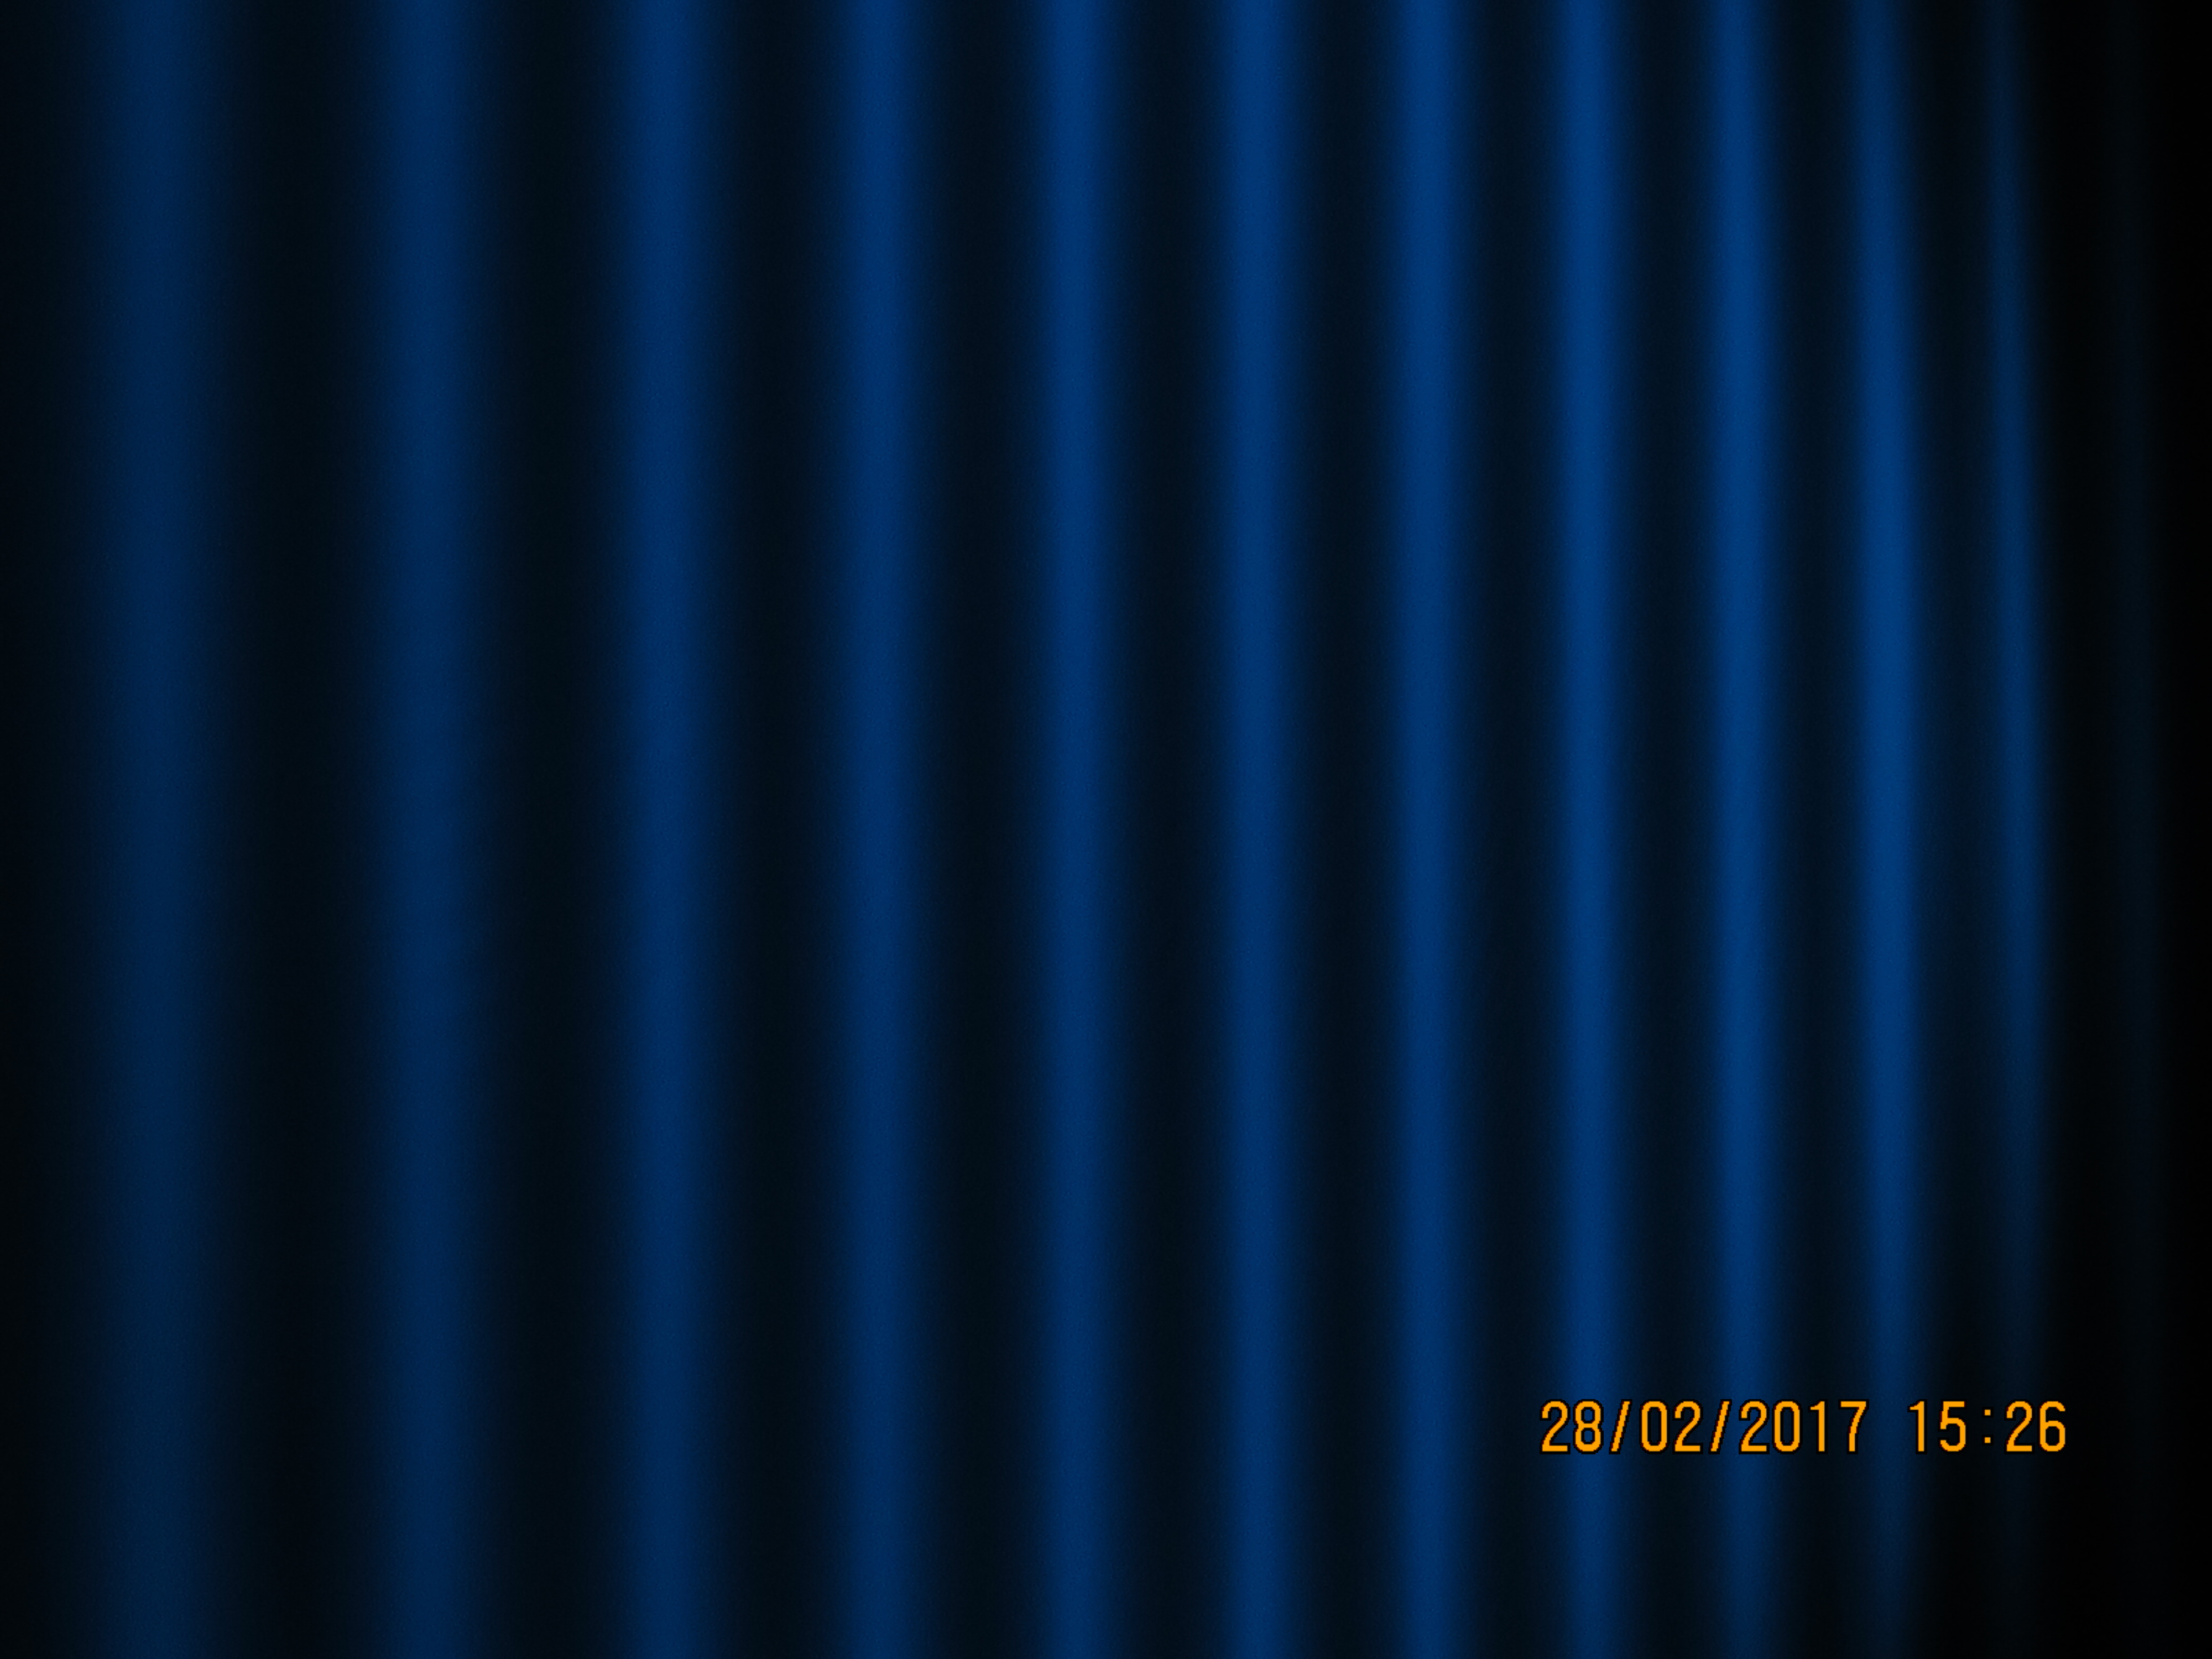
\includegraphics[width=\linewidth]{images/blau_oM.jpg}
		\centering
		a) B = $\SI{0}{\tesla}$
	\end{minipage}
	\begin{minipage}[t]{0.6\textwidth}
		
\includegraphics[width=\linewidth]{images/blau_sigma.jpg}
		\centering
		b) B = $\SI{314.06}{\milli\tesla}$
	\end{minipage}}
	\captionof{figure}{Interferenzmuster der Lummer-Gercke-Platte für die $\sigma$-Übergänge der Cd-Spektrallinie bei $\lambda=\SI{480.0}{\nano\metre}$, mit a) ohne Magnetfeld und b) mit Magnetfeld}
	\label{fig:blau_sigma}
	\vspace{0.5cm}

In Tabelle \ref{tab:blausigmamessung} sind die aus Abbildung \ref{fig:blau_sigma} abgelesenen Werte für $\delta s$ und $\Delta s$ sowie die daraus berechneten Wellenlängenänderungen dargestellt.
\begin{table}[H]
	\centering
	\captionof{table}{Abstände $\Delta s$ und $\delta s$ der Interferenzstreifen mit Wellenlängenänderung für die $\sigma$-Übergänge der Cd-Spektrallinie bei $\lambda=\SI{480.0}{\nano\metre}$}
	\label{tab:blausigmamessung}
	\begin{tabular}{r r r r}
			\toprule
			Ordnung n & $\Delta s$/px & $\delta s$/px & $\delta \lambda$/pm \\
			\midrule
			0 & 472 & 288 & 8.21 \\
			1 & 424 & 243 & 7.71 \\
			2 & 378 & 204 & 7.26 \\
			3 & 350 & 190 & 7.30 \\
			4 & 332 & 180 & 7.29 \\
			5 & 303 & 160 & 7.10 \\
			6 & 285 & 156 & 7.36 \\
			7 & 274 & 138 & 6.77 \\
			8 & 244 & 134 & 7.39 \\
			9 & 202 & 126 & 8.39 \\
			\bottomrule
	\end{tabular}
\end{table}
Der über mehrere Ordnungen gemittelte Wert der Wellenlängenänderung beträgt
\begin{align}
\delta \lambda = \SI{7.48(16)}{\pico\metre}\,.
\end{align}
\subsubsection{$\pi$-Übergänge für $\lambda=\SI{480.0}{\nano\metre}$}

\noindent\makebox[\textwidth][c]{
	\begin{minipage}[t]{0.6\textwidth}
		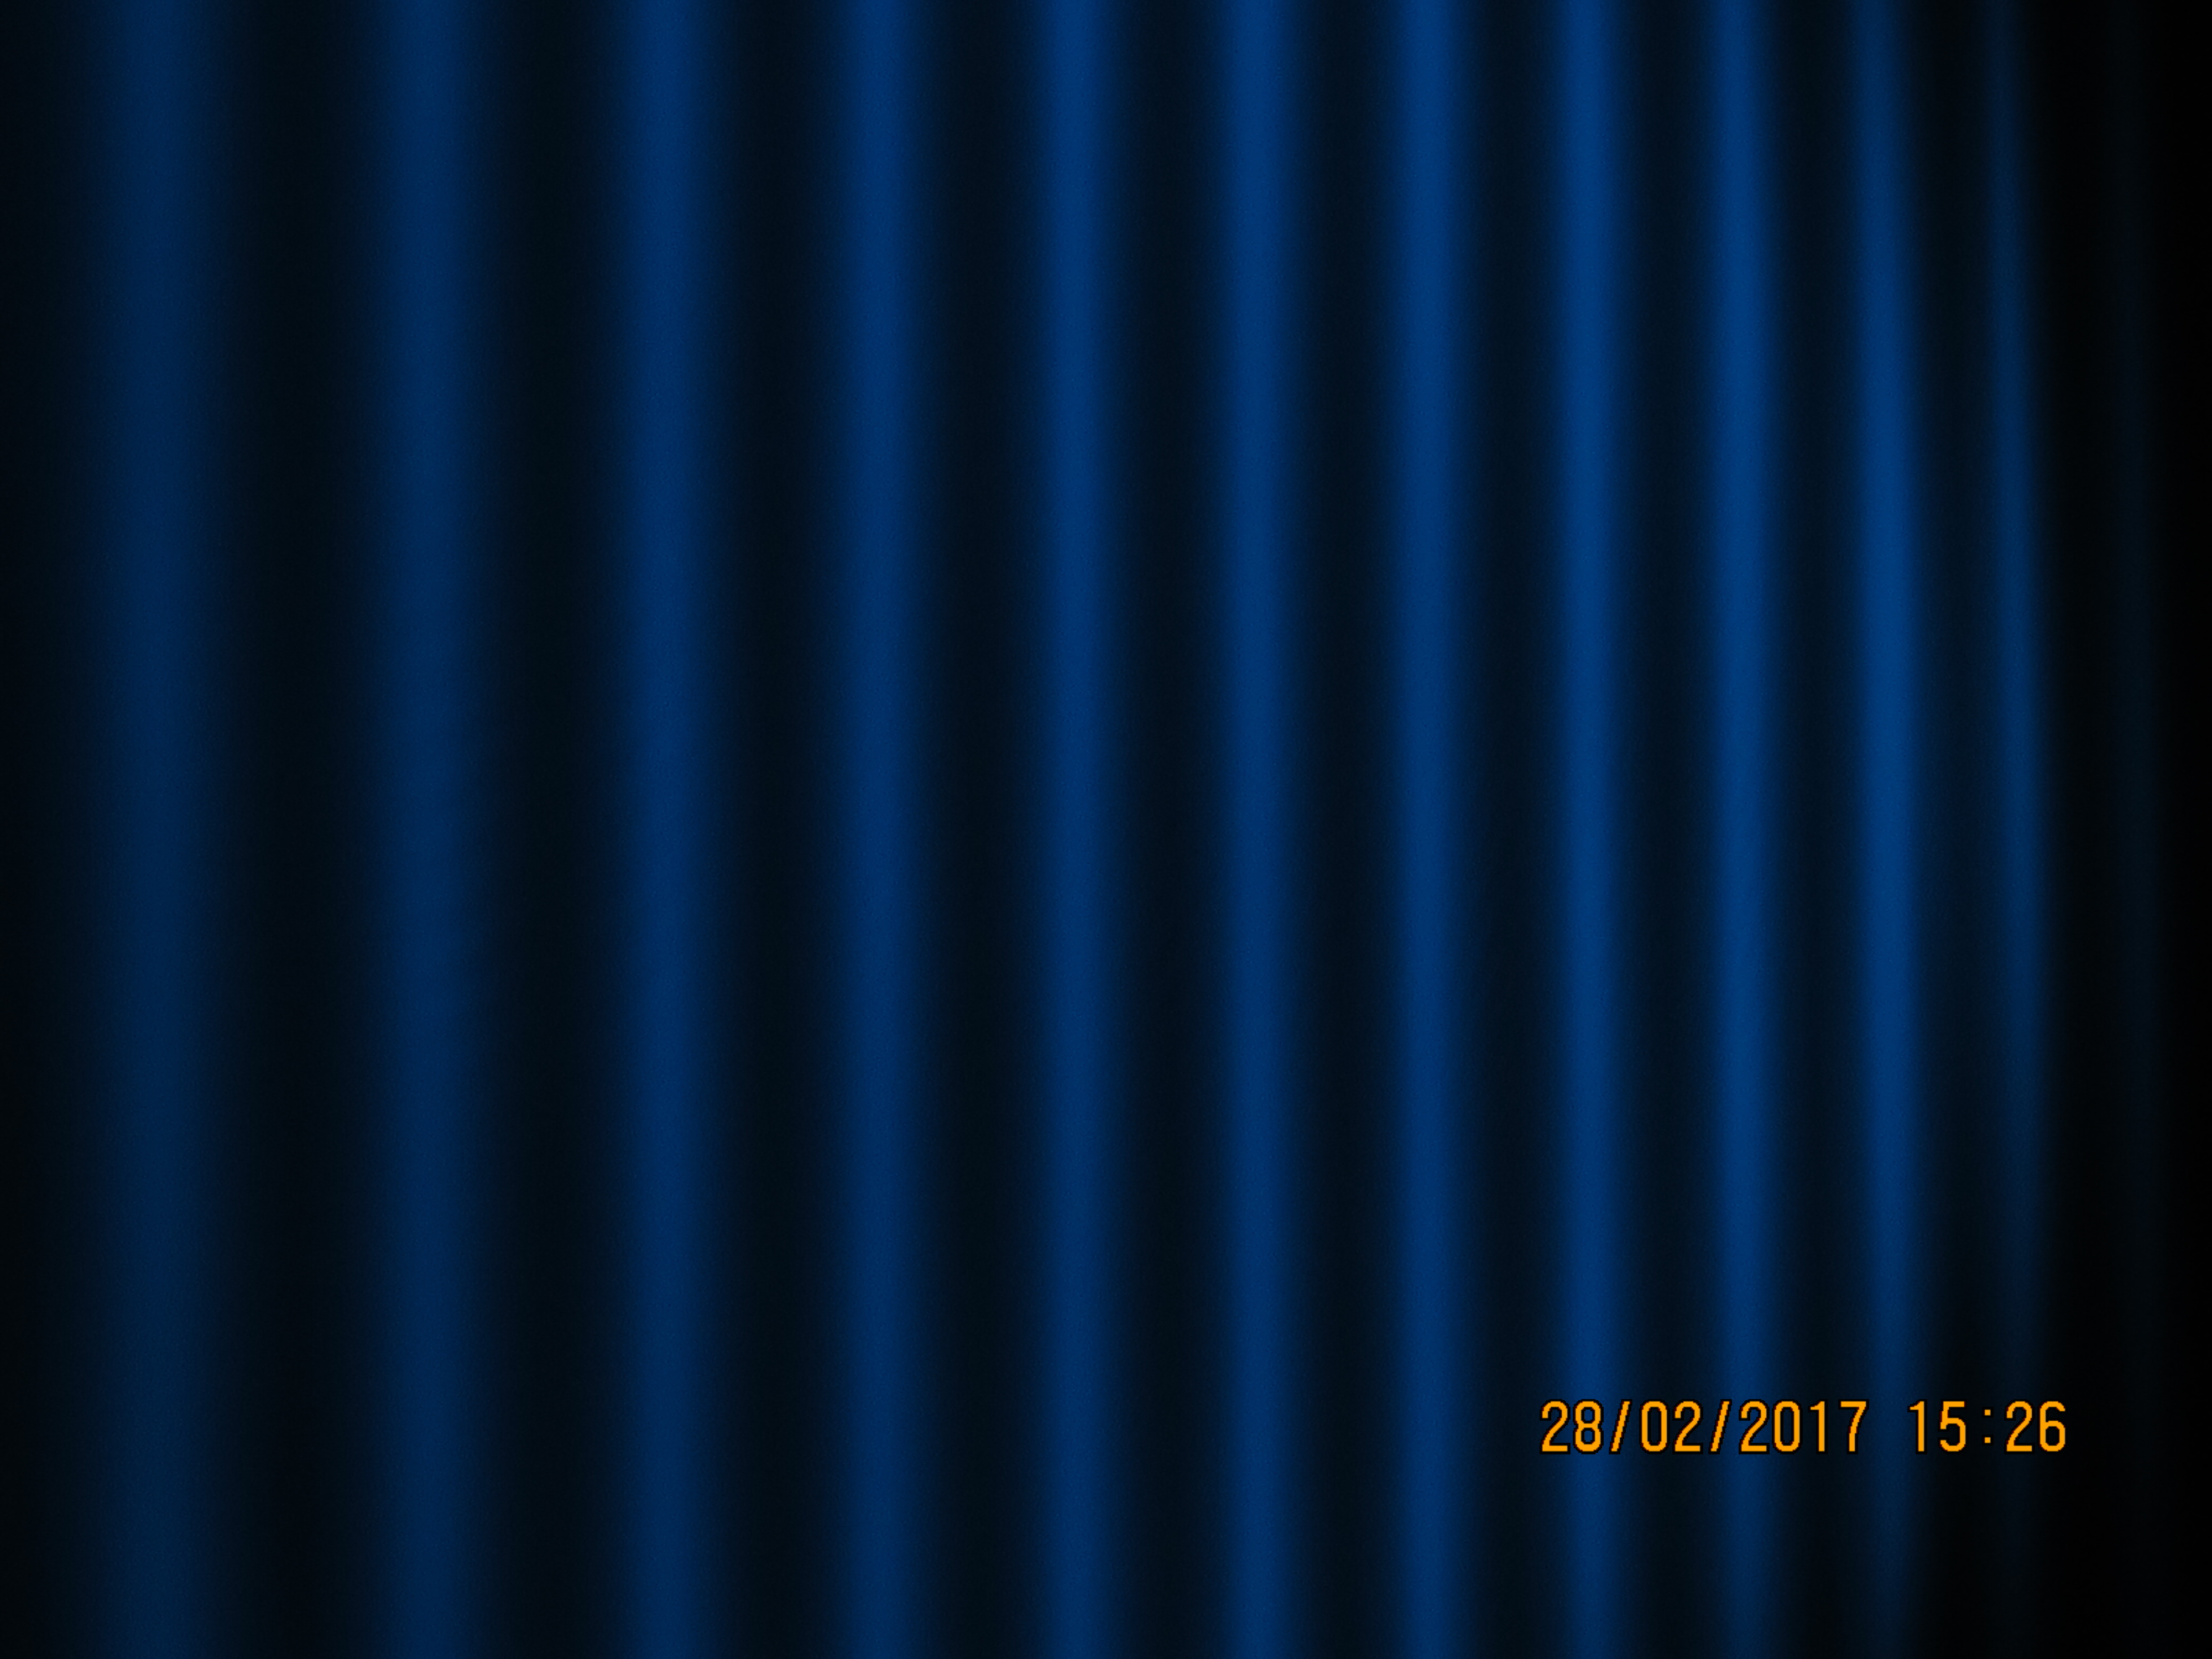
\includegraphics[width=\linewidth]{images/blau_oM.jpg}
		\centering
		a) B = $\SI{0}{\tesla}$
	\end{minipage}
	\begin{minipage}[t]{0.6\textwidth}
		
\includegraphics[width=\linewidth]{images/blau_pi.jpg}
		\centering
		b) B = $\SI{957.54}{\milli\tesla}$
	\end{minipage}}
	\captionof{figure}{Interferenzmuster der Lummer-Gercke-Platte für die $\pi$-Übergänge der Cd-Spektrallinie bei $\lambda=\SI{480.0}{\nano\metre}$, mit a) ohne Magnetfeld und b) mit Magnetfeld}
	\label{fig:blau_pi}
	\vspace{0.5cm}

In Tabelle \ref{tab:blaupimessung} sind die aus Abbildung \ref{fig:blau_pi} abgelesenen Werte für $\delta s$ und $\Delta s$ sowie die daraus berechneten Wellenlängenänderungen dargestellt.
\begin{table}[H]
	\centering
	\captionof{table}{Abstände $\Delta s$ und $\delta s$ der Interferenzstreifen mit Wellenlängenänderung für die $\pi$-Übergänge der Cd-Spektrallinie bei $\lambda=\SI{480.0}{\nano\metre}$}
	\label{tab:blaupimessung}
	\begin{tabular}{r r r r}
		\toprule
		Ordnung n & $\Delta s$/px & $\delta s$/px & $\delta \lambda$/pm \\
		\midrule
		0 & 472 & 224 & 6.38 \\
		1 & 424 & 212 & 6.73 \\
		2 & 378 & 164 & 5.84 \\
		3 & 350 & 152 & 5.84 \\
		4 & 332 & 136 & 5.51 \\
		5 & 303 & 130 & 5.77 \\
		6 & 285 & 122 & 5.76 \\
		7 & 274 & 114 & 5.60 \\
		8 & 244 & 106 & 5.84 \\
		9 & 202 & 100 & 6.66 \\
		\bottomrule
	\end{tabular}
\end{table}
Der über mehrere Ordnungen gemittelte Wert der Wellenlängenänderung beträgt
\begin{align}
\delta \lambda = \SI{5.99(14)}{\pico\metre}\,.
\end{align}
\subsection{Bestimmung der Landé-Faktoren}
Aus der Wellenlängenänderung können mit der Energieverschiebung $\Delta E$ die Landé-Faktoren $g_{ij}$ berechnet werden. \\
Dazu wird die der Zusammenhang
\begin{align*}
E=\frac{hc}{\lambda}
\end{align*}
verwendet, sodass sich die Energieverschiebung aus
\begin{align}
\Delta E = \left| \frac{\partial E}{\partial \lambda}\delta \lambda\right| = \frac{hc\delta \lambda}{\lambda ^2}
\end{align}
ergibt. Für die Landé-Faktoren ergibt sich damit
\begin{align}
\left| g_{ij}\right| =\frac{\Delta E}{\mu_B B}=\frac{hc}{\lambda ^2\mu_B B}\delta \lambda\,.
\end{align}
Die aus den Messdaten berechneten Wellenlängenänderungen sowie die daraus berechneten Landé-Faktoren sind in Tabelle \ref{tab:lande} dargestellt.

\begin{table}[H]
	\centering
	\captionof{table}{Wellenlängenänderungen $\delta \lambda$ sowie daraus berechnete Landé-Faktoren $g_{ij}$}
	\label{tab:lande}
	\begin{tabular}{r r r r}
		\toprule
		$\lambda$/nm & Polarisierung & $\delta \lambda$/pm & $\left| g_{ij}\right|$ \\
		\midrule
		643.8 & $\sigma$ & $10.28\pm0.04$ & $1.53\pm0.01$ \\
		480.0 & $\sigma$ & $ 7.48\pm0.16$ & $1.23\pm0.03$ \\
		480.0 & $\pi$	 & $ 5.99\pm0.14$ & $0.32\pm0.01$ \\
		\bottomrule
	\end{tabular}
\end{table}
		
\section{Diskussion}
In Tabelle \ref{tab:literatur} sind die experimentell ermittelten Landé-Faktoren, die Theoriewerte sowie   dargestellt.
\begin{table}[H]
	\centering
	\captionof{table}{Vergleich von experimentell bestimmten Landé-Faktoren mit Theoriewerten}
	\label{tab:literatur}
	\begin{tabular}{r r r r r}
		\toprule
		$\lambda$/nm & Polarisierung & $\left| g_{ij}\right|_{exp}$ & $\left| g_{ij}\right|_{theo}$ & $\delta \left|g_{ij}\right|$ \\
		\midrule
		643.8 & $\sigma$ &  $1.53\pm0.01$ & 1 & 53.0\% \\
		480.0 & $\sigma$ &  $1.23\pm0.03$ & 2 & 38.5\% \\
		480.0 & $\pi$	 &  $0.32\pm0.01$ & 0.5 & 36.0\% \\
		\bottomrule
	\end{tabular}
\end{table}
Die experimentell bestimmten Werte der Landé-Faktoren weichen stark von den Theoriewerten ab, die Abweichungen reichen dabei von 36.0\% für den $\pi$-Übergang bei $\lambda=\SI{480.0}{\nano\metre}$ bis zu 53.0\% für den $\sigma$-Übergang bei $\lambda=\SI{643.8}{\nano\metre}$. Ursachen dafür können die ungenaue Bestimmung des Magnetfeldes sowie ein systematischer Fehler im Aufbau sein. \\
Desweiteren können die Verschiebungen aufgrund des geringen Kontrastes nur wenig genau abgelesen werden, was eine hohe Ungenauigkeit bei der Berechnung der Landé-Faktoren zur Folge hat.

\section{Quellen}
%\renewcommand{\labelenumi}{\value{enumi}}
\begin{enumerate}[label={[\arabic*]}]
\item \label{q:anleitung} \textbf{Physikalisches Praktikum}, TU Dortmund: \\
\textit{Versuchsanleitung zu Versuch: V27 Der Zeeman-Effekt} \\
\url{http://129.217.224.2/HOMEPAGE/PHYSIKER/MASTER/SKRIPT/V27.pdf} (letzte Version vom 27.03.2017, 09:07
\end{enumerate}

\end{document}
